\documentclass[10pt]{report}
\usepackage{lmodern}
\usepackage[scaled]{helvet}
\renewcommand*\familydefault{\sfdefault} 
\usepackage[T1]{fontenc}
\usepackage{courier}
\usepackage[utf8]{inputenc}
\usepackage{amsmath,amsthm,amsfonts,amssymb,amscd}
\usepackage[a4paper,hmargin=0.8in,bottom=1.3in]{geometry}
\usepackage{lastpage,enumerate,fancyhdr,mathrsfs,xcolor,listings,graphicx,hyperref,enumitem}
\lstset{basicstyle=\footnotesize\ttfamily}
\lstset{
escapeinside={/*!}{!*/}
}
\title{Operating Systems: Shortnotes}
\author{Hardik Rajpal}
\begin{document}
\maketitle
\tableofcontents
\pagebreak
\chapter{Introduction}
\chapter{CPU Virtualization}
\section*{Terms}
\begin{itemize}
\item Process Control Block: A per-process data structure that tracks process meta-data.
\end{itemize}
\chapter{Memory Virtualization}
\section*{Terms}
\begin{enumerate}
    \item Address Space: The running program's view of the memory available to it. Every program only sees the memory available to it, which is split between the code, (static) data, heap and stack.
    \item Sparse Address Space: An address space where most of the
    memory between heap and stack is unused.
    \item Memory Management Unit: The hardware responsible for V2P translation.
    \item Protection Bits: Bits in VA that represent the process'
    access permission for the PA to which it points, including read/write/execute permissions. 
    \item Fragmentation: Wastage of physical memory space.
    \begin{itemize}
        \item Internal: Wastage within a contiguous block of physical memory allocated to a process. An example is the unused space between heap and stack in a simple base-bounds V2P map.
        \item External: Wastage outside of contiguous blocks that have been allocated. This is because of the gaps of available physical memory being too small to fit any new contiguous segments. 
    \end{itemize}
    \item Page: Unit of address space.
    \item Page Frame: Unit of physical address space to which a page can be mapped. Same unit, but \textbf{pages} exist in the
    virtual address space whereas \textbf{page frames} exist
    in the physical address space.
    \item Spatial Locality: nearby instructions (in the control flow) access nearby memory locations.\\ Ex. with code for sequential array processing.
    \item Temproal Locality: nearby instructions (in the control flow) accessing a single memory address repeatedly.
\end{enumerate}
\section{Address Space}
The program is actually loaded into random physical addresses, but due to the address space
abstraction, the program sees the memory available to it as a contiguous chunk, starting at 0.
Every address the program sees is virtual and the OS (with some translation mechanism
of the VA to PA) uses the PA whenever the program references the VA.
\section{Address Translation}
All address translation is hardware-based for efficiency.
Each memory access (load/store) is intercepted by the hardware
and the VA is translated to a PA. The OS helps setup the
hardware for the right translation (per process), and manages memory.
\subsection{Dynamic Relocation a.k.a. (Base, Bound)}
\begin{itemize}
\item Two registers for this in the CPU: base and bound.
\item Translation:
\begin{lstlisting}
V2P(VA v){
    if(v > bound || v < 0){
        throw "Out of Bounds";
    }
    return (base + v);
}
\end{lstlisting}
\item Values of base and bounds for each process are stored in its
PCB.
\item Base and bound registers are privileged: if access is attempted
from user mode, the OS terminates the access-requesting process.
\end{itemize}
\subsection{Segmentation}
\begin{itemize}
\item Generalized base and bounds for each logical segment
of each process: code, heap and stack.
\item Maintain base and size for each segment:
\begin{center}
    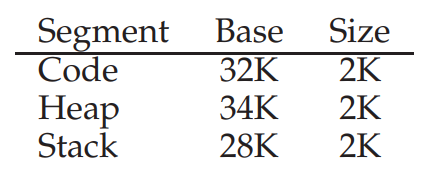
\includegraphics[width=5cm]{res/segmentation.png}
\end{center}

\item Use VA[0:2] to represent the segment type.
\item Better handles \textbf{sparse address spaces}, where
the program often has very little heap and stack data and
thus a lot of the in-between space in a contiguous allocation is 
wasted.
\item Translation is more involved:
\begin{lstlisting}
V2P(VA v){
    segment = v[0:2];//or bit operations.
    offset = v[2:];//or bit operations.
    if(offset < 0 || offset > segdata[segment]["bound"]){
        throw "Out of Bounds"
    }
    else{
        return segdata[segment]["base"] + offset;
    }
}
\end{lstlisting}
\item OS responsibilities:
\begin{itemize}
    \item On each context switch the \textbf{segmentation table} for the process is replaced by the incoming process' table.
    \item On a receiving new process (and its accompanying address 
    space), the OS has to find space in the physical memory for its 
    segments. If the segments are of varying sizes (bounds) this is more involved.
    \item Variable size segments lead to external fragmentation.
    \item A solution to external fragmentation is periodic compaction:
    \begin{enumerate}
        \item Stop running processes.
        \item Copy their data to a contiguous chunk of memory.
        \item Update their segment register values.
    \end{enumerate}
    This creates available contiguous chunks of physical memory but 
    compaction is expensive (copying segments is memory-intensive)
    and would take up a fair amount of CPU time.
    \item Alternative approaches involve using a free-list 
    management algorithm like:
    \begin{itemize}
        \item best-fit
        \item worst-fit
        \item first-fit
        \item buddy algorithm
    \end{itemize} 
    \item External fragmentation will always exist in this scheme,
    however. The algorithms above simply aim to minimize it. The real solution is to disallow variable sized segments.
\end{itemize}
\item Some systems merge code and heap segments to use only one bit
to represent segment.
\item There are \textbf{implicit} approaches to identify the segment too, where the program infers the segment by identifying how the 
VA was conceived:
\begin{itemize}
    \item from a PC $\implies$ use code segment.
    \item from ebp $\implies$ use stack segment.
    \item else, use heap segment.
\end{itemize}
\item We also need an additional bit to identify the direction of growth of the segment, if this varies across the segments. The translation function is modified to take this into account.
\end{itemize}
\subsubsection{Sharing Segments}
\begin{itemize}
\item With some VA bits used to represent permissions that a process
has for the segment \textbf{protection bits}, we can factor include segments with varying
permissions.
\item Translation function is appropriately modified to 
raise an exception whenever a process attempts to violate
permissions for a PA.
\item Read-only code can be shared across multiple processes, without
the worry of harming isolation.
\end{itemize}
\subsubsection{Fine-grained Vs. Coarse-grained}
\begin{itemize}
\item Segments of code, heap and stack are relatively large (coarse-grained segmentation).
\item Fine-grained segmentation further splits up each
of these logical segments and identifies each segment using
a \textbf{segment table}. This allows for better memory
management by the OS (by moving unused segments to disk).
\end{itemize}
\subsection{Paging}
\begin{itemize}
\item Split the address space (abstraction visible to the process) 
into fixed-size units called pages. The corresponding contiguous units in the physical address space are called page frames.
\item To record each page's mapping for each process, the OS
maintains a \textbf{page table} per process that is pointed to by the \textbf{Page Table Base Register (PTBR)}.
\item Translation: (neglecting bits other than VPN and offset)
\begin{center}
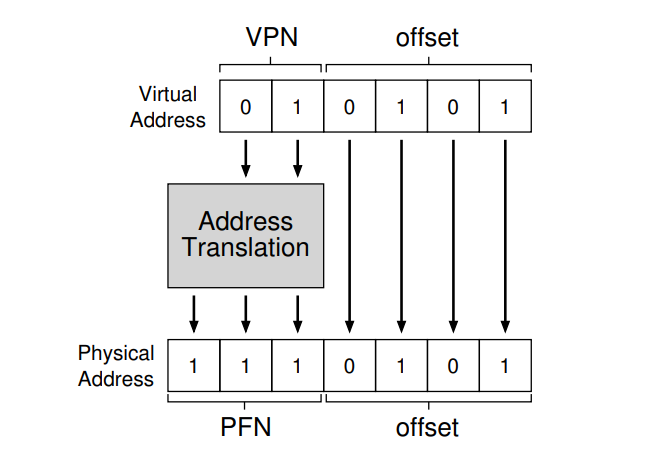
\includegraphics[width=5cm]{res/paging.png}
\end{center}
\end{itemize}

\subsubsection{Inside The Page Table}
\begin{itemize}
\item The OS stores the page table in memory, in units of
\textbf{page table entries} (PTEs) because of the sheer size of page tables.
\item Each PTE has a physical address to which it maps and a collection of metadata bits.
\item The PTEs are stored in a (nested) array-like structure, such
that a VPNs can be used as indices into the structure, pointing
at the PTE that contains their corresponding PFN.
\item The metadata bits:
\begin{enumerate}
    \item Valid bit:indicates whether PTE is valid.
    \begin{itemize}
        \item When a program starts running, all the (virtual) space 
        between the heap and stack is unused and hence unmapped. 
        Hence entries at pagetable [VA] for those addresses are 
        invalid.
        \item If a program tries to access invalid memory, a trap is
        generated and the program is likely terminated.
        \item The valid bit is crucial for supporting \textbf{sparse address spaces}.
        \item Invalid PTEs don't have any physical memory mapped to 
        them, this lets us use only the physical memory we need.
    \end{itemize}
     \item Protection bits: indicate whether the page can be
     read from, written to or executed from. Invalid accesses
     generate a trap to the OS.
     \item Present bit: indicates whether page is present in memory
     (or has been swapped out to disk).
     \item Dirty bit: indicates whether the page has been modified 
     since being loaded into memory.
     \item Reference (a.k.a. accessed) bit: used to track if the
     page has been accessed since the bit was last reset. This 
     information helps in page replacement, to keep popular pages
     around.
     \item User/Supervisor bit: indicates if processes can access
     the page in user mode.
     \item Hardware caching bits: help determine how hardware caching works for the page. 
\end{enumerate}
\end{itemize}
\subsubsection{How It Works}
When the OS reads a command to access/write to a memory location at \texttt{VA0},
\begin{enumerate}
    \item Extract \texttt{VPN} and \texttt{offset} from \texttt{VA0}.
    \item Access \textbf{PTE} stored at \texttt{PTBR + VPN}. \hfill \textbf{Memory Access 1 (PTE read)}
    \item Extract the \texttt{PA} and \textbf{permission bits} from \textbf{PTE}.
    \item Verify \textbf{permission bits}.
    \begin{itemize}
        \item If page is invalid, raise \texttt{Segmentation Fault} exception.
        \item If permissions are insufficient, raise \texttt{Protection Fault} exception. 
    \end{itemize}
    \item Read/write to data stored at \texttt{PA + offset}. \hfill \textbf{Memory Access 2 (Data access)}
\end{enumerate}
\subsubsection{Making Paging Faster}
The procedure given above is without the use of \hyperref[subsec:TLB]{TLBs}, which are always used in the real world to speed up paging. 
\subsubsection{Reducing The Page Table's Size}
\begin{enumerate}
\item Increase Page Size: the factor by which the page size is increased is the factor by which the page table's size is reduced.
\begin{itemize}
\item This approach is commonly used by DBMSs and other high-end
commercial applications. However, their goal is to reduce pressure
on the TLB by reducing the number of translations, instead of minimizing the page table's size.
\item The major problem with this is internal fragmentation. Hence, it's only suitable if the programs are guaranteed to use the
large pages allocated to them almost thoroughly.
\end{itemize}
\item  Hybrid approach: Paging + Segments
\begin{itemize}
    \item We first note that in each table, most of the PTEs are 
    invalid, and only a select few are mapped to physical page 
    frames.
    \item This approach involves maintaining a separate page table
    for the code, stack and heap segments of the virtual address 
    space.
    \item We have base and bound registers for each segment as before, except that the \textbf{base}
    points to the physical address of the page table of that segment.
    \item Note that all six registers must be updated on a context
    switch.
    \item The translation involves:
    \begin{lstlisting}
    V2P(VA v){
        segment = v[0:2];//or bit operations.
        VPN = v[2:k];//or bit operations.
        offset = v[k:];//or bit operations.
        addressOfPTE = Base[segment] + (VPN*sizeof(PTE));
        PTE = read(addressOfPTE);
        PFN = PTE[:c]
        PA =  PFN + offset;
        return PA;
    }
    \end{lstlisting}
    \item However, like segmentation, (i) this method can't help 
    with 
    the wastage of memory due sparse usage within segments (ex. a 
    sparsely used heap), and (ii) leads to external fragmentation, 
    as the variable sized page tables need to be allocated 
    contiguous chunks of memory.
\end{itemize}
\item Multi-level page tables:
\end{enumerate}
\subsubsection{Advantages of paging}
\begin{itemize}
    \item Flexibility is an important advantage of paging: it works 
    regardless of how the process uses the address space, how the heap and stack grow or how they are used.
    \item Flexibility also ensures it can handle sparse address spaces and minimize internal fragmentation.
    \item Simplicity: when new pages are requested, the OS simply
    traverses a free list and returns the first pages that it finds.
    \item It avoid external fragmentation altogether by having fixed-size units.
\end{itemize}
\subsection{TLB}
\begin{itemize}
    \item It's a part of the MMU and is a hardware cache of popular V2P translations.
    \item The process of memory access with the TLB is:
    \begin{enumerate}
    \item Extract \texttt{VPN} and \texttt{offset} from \texttt{VA0}.
    \item If TLB has an entry for \texttt{VA0} (TLB hit)
    \begin{itemize}
        \item If permissions are insufficient, raise \texttt{Protection Fault} exception.
        \item Extract \texttt{PA} for \texttt{VA} from TLB.
        \item Read/write to data at \texttt{PA + offset}. \hfill \textbf{Memory Access 1 (Data access)}
    \end{itemize}
    \item Otherwise, carry out steps 2, 3 and 4 of the usual access routine. \hfill \textbf{Memory Access 1 (PTE read)}
    \item Instead of step 5, insert the translation \texttt{(VPN,PA,Protection Bits)} into the TLB.
    \item Retry the memory access instruction (start at 1 of this sequence).
    \end{enumerate}
    \item Like most caches, TLB is built on the premise that most 
    translations are found in the cache (hits). The little overhead 
    costs of using a TLB (little because it's near the processing 
    core and designed to be quite fast), are made up for by the hit cases. 
    \item The speed of a cache comes partly from its minimal size; any large cache is by definition slow.
\end{itemize}
\subsubsection{TLB Misses}
\begin{itemize}
\item We say a program exceeds the TLB coverage if it generates
a large number of TLB misses, by accessing (in a short period of time) more pages than the number of translations the TLB can fit.
\item One solution to this is to allow larger pages for storing
key data structures that such programs access repeatedly, and thus
allowing a single translation in the TLB to serve many memory accesses.
\item Support for large pages is often exploited by programs such as DBMSs, which have large and randomly accessed data structures.
\item In CISC computers, the hardware would handle the TLB miss entirely (low trust on the OS designers).
\item With physically-indexed caches, some translation of the VA has to take place for the lookup itself, and thus they are very slow. Check cache notes if any.
\\On a miss,
\begin{itemize}
    \item The hardware would walk the page table using \texttt{PTBR} to get the \texttt{PA} for the \texttt{VPN} that induced a miss.
    \item It would update the TLB with the new translation.
    \item Then hit retry on the instruction that resulted in a TLB miss.
\end{itemize}
\item In RISC computers, the TLB is software-managed. On a TLB miss, the hardware just raises an exception (\texttt{TLB\_MISS}).
\item With software-managed TLBs, it is important that the instructions provided by the hardware to read/write to the TLB,
are only allowed to be run in privileged modes.
\begin{enumerate}
\item This pauses the current instruction stream, raises the privilege level to kernel mode and jumps to a \textbf{trap handler}.
\item The targeted code looks up the translation in the page table, uses \textbf{privileged} instructions to update the TLB, and returns from the trap.
\end{enumerate}
Note that:
\begin{itemize}
    \item Note that on return the execution must pick up \textbf{at the causal instruction} that caused the trap, instead of the usual return-from-trap where execution picks up \textbf{after the causal instruction.}
    \item While accessing the code for trap handler for \texttt{TLB\_MISS}, the OS should not incur a TLB miss, which would imply an infinite chaing of TLB misses. To avoid this, we can:
    \begin{enumerate}
        \item Keep TLB miss handlers in \textbf{unmapped} physical memory, so that their execution does not involve address translation (and hence TLBs).
        \item Reserve entries in TLB for permanently-valid (\textbf{wired}) translations and use some of these slots for the trap-handler code's memory address' translation.
    \end{enumerate}
\end{itemize}
\item The advantage of a software-managed TLB include:
\begin{itemize}
    \item Flexibility: the OS 
    can store the PTEs in any data structure it wants, as it's 
    allowed to update the page table walk function, since it's not 
    burned into a chip.
    \item Simplicity: the hardware just has to raise an exception and relies on the OS to resolve the TLB miss. 
\end{itemize} 
\end{itemize}
\subsubsection{TLB Contents}
\begin{itemize}
    \item The TLB has 32/64/128 entries and is \textbf{fully associative} ($\equiv$ any translation can be anywhere in the TLB, and the hardware searches the entire TLB in parallel to find the entry for \texttt{VPN}).
    \item The TLB entry has: VPN $|$ PFN $|$ other bits.
    \item The other bits are:
        \begin{itemize}
            \item Valid bit: denoting if \textbf{the TLB entry is valid, NOT the page.}
            \item Protection bits.
            \item Global bit, to indicate globally shared translations. If this is set, ASID bit is ignored.
            \item Address-space identifier (ASID) (to identify if the entry is for the given process or in a shared region).
            \item Dirty bit, to indicate if the page has been modified since it was brought into memory.
            \item Coherence bits: they determine how a page is cached by the hardware.
            \item Page mask field: to support multiple page sizes.
        \end{itemize}
    \item On a context switch, the OS must ensure one processes translations in the TLB are not used by another process (unless it's a shared memory region). This can be done via:
    \begin{enumerate}
    \item Simply flushing the TLB on a context switch (marking each entry as invalid). This can be coded up in the OS or the hardware
    can be set to flush the TLB whenever the PTBR is updated.
    \item Maintain ASID for each entry and a privileged register to hold the ASID of the current process. Note that ASIDs require much fewer (8ish bits) as compared to PIDs (32ish bits).\\
    Additionally, ASIDs (along with the permission bits) enable sharing of code pages across processes.
    \end{enumerate}
\end{itemize}
\label{subsec:TLB}
\subsubsection{Replacement Policy}
We want to maximize the hit-rate in the TLB based on our 
choice of a replacement policy. Some common choices are:
\begin{enumerate}
\item Evict Least Recently Used entry: relies on temporal locality 
of address usage. The least recently used entry in the cache will
probably not be used any time soon, as future access will be closer
to the more recent accesses in the cache.
\item Random: Avoids making corner-case worst-possible decisions all 
the time. (For example, a for loop which requires TLB eviction, with the LRU policy in place.) 
\end{enumerate}
\section{Free Space Management}
\chapter{Concurrency}
From Neso Academy's OS lectures.
\section{Basics of Threads}
\begin{itemize}
\item Each program may have multiple processes associated with it. Each process may have multiple threads; threads are a basic unit of execution or CPU utilization.
\item A thread comprises of:
\begin{enumerate}
\item A thread ID
\item A program counter
\item A register set
\item A stack.
\end{enumerate}
\item Threads of the same process share:
\begin{enumerate}
\item Code section
\item Data section
\item Other OS resources, such as files and signals.
\end{enumerate}
\item A \textbf{traditional/heavyweight} has a single thread of control. Having multiple threads of control allows a process to perform multiple tasks at a time.
\begin{center}
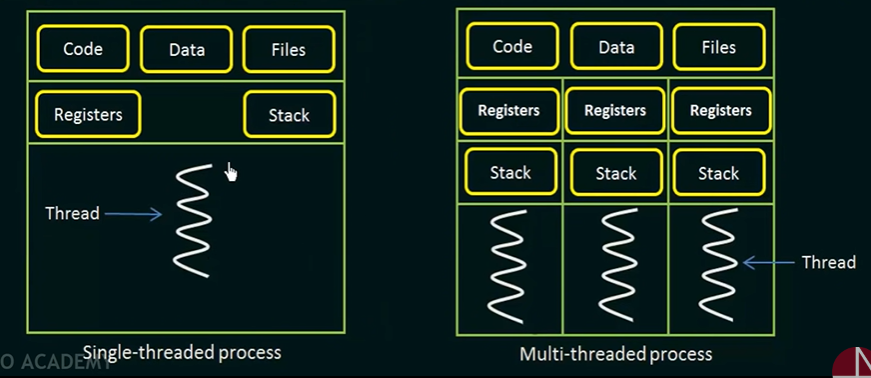
\includegraphics[width=11cm]{res/threads.png}
\end{center}
\item The benefits of multithreaded programming are:
\begin{enumerate}
\item \textbf{Responsiveness}: interactive applications allow a program to continue running even one of its tasks is blocked in its thread in a lengthy operation, thereby allowing responsiveness.
\item \textbf{Resource Sharing}: Code, data and files are shared between threads, allowing for better utilization of system resources.
\item \textbf{Economy}: Saves the costs of allocating a separate process for each task.
\item \textbf{Utilization of Multiprocessor Arch.}: Multithreading on a multi-CPU machine increases concurrency by using parallelism.
\end{enumerate}
\end{itemize}
\section{Multithreading Models and Hyperthreading}
\begin{itemize}
\item There are two types of threads:
\begin{enumerate}
\item User threads: Supported above the kernel and are managed without kernel support.
\item Kernel threads: Supported and managed directly by the OS.
\end{enumerate}
\item Multithreading models describe the type of relations between user and kernel threads. There are three common types:
\begin{enumerate}
\item Many-to-One
\item One-to-One
\item One-to-Many
\end{enumerate}
\end{itemize}
\subsection{Many-to-One}
\begin{itemize}
\item Many user-level threads are mapped to a single kernel thread.
\item Thread management is done by the thread library in user space; thus, it is efficient.
\item The limitations are:
\begin{enumerate}
\item The entire process will block if a thread makes a system call.
\item Since only one thread can access the kernel at a time, multiple threads are unable to run in parallel on multiple processors.
\end{enumerate}
\end{itemize}
\subsection{One-to-One}
\begin{itemize}
\item A bijection between user-level and kernel-level threads.
\item Provides more concurrency than the many-to-one model by allowing another thread to run when a thread makes a blocking system call.
\item Also allows multiple threads to run in parallel on multiple processors.
\item The limitations are:
\begin{enumerate}
\item Creating a user thread requires creating a corresponding kernel thread, which is costly.
\item The overhead of creating kernel threads can burden the performance of an application; most implementations of this model restrict the number of threads supported by the system.
\end{enumerate}
\end{itemize}
\subsection{Many-to-Many}
\begin{itemize}
\item Each user thread is mapped to many shared kernel threads. \# kernel threads $\le$ \# user threads.
\item The number of kernel threads may be specific to a particular application or machine.
\item Developers can create as many user threads as necessary, and the corresponding kernel threads can run in parallel on a multiprocessor.
\item Blocking system calls result in the kernel scheduling another thread for execution.
\item This model makes the best of the previous two models and is what is implemented in most systems.
\item However, with its difficulty of implementation and increasing number of cores, one-to-one is increasingly preferred.
\end{itemize}
\section{Hyperthreading a.k.a. Simultaneous Multithreading (SMT)}
\begin{itemize}
\item Multiple multithreaded programs running at the same time.
\item Hyperthreaded systems allow their processor cores' resources to become multiple logical processors for performance.
\item In hyperthreading, physcial cores are logically divided into multiple virtual cores, to support multiple threads running concurrently.
\item It enables the processor to execute two (or more) threads, sets of instructions, at the same time.
\item Hyperthreading allows two streams to be executed concurrently, it s like having two separate processors working together.
\end{itemize}
\section{Notes from Interview Questions}
\chapter{Misc.}
\chapter{References}
\begin{enumerate}
\item OSTEP
\end{enumerate}
\end{document}